\chapter{Конструкторский раздел}
\label{cha:design}
\section{Оценка качества изображений}
\subsection{PSNR}
Пиковое отношение сигнала к шуму (англ. peak signal-to-noise ratio) - соотношение между максимумом возможного значения сигнала и мощностью шума, искажающего значения сигнала.\cite{Habr1} 
\begin{equation}
PSNR=20\log_{10} \frac{MAX_i}{\sqrt{MSE}} 
\label{F:F1}
\end{equation}
Где $MAX_i$ - это максимальное значение, принимаемое пикселем изображения, MSE - среднеквадратичное отклонение.  Для двух монохромных изображений I и K размера m×n, одно из которых считается зашумленным приближением другого, вычисляется так:
\begin{equation}
MSE =\frac{1}{m*n}\sum_{i=0}^{m-1}\sum_{j=0}^{n-1}|I(i,j)-K(i,j)|^2
\label{F:F2}
\end{equation}
\subsection{SSIM}
Индекс структурного сходства (SSIM от англ. structure similarity) — метод измерения схожести между двумя изображениями путем полного сопоставления. SSIM-индекс является развитием традиционных методов, таких как PSNR (peak signal-to-noise ratio) и метод среднеквадратичной ошибки MSE, которые оказались несовместимы с физиологией человеческого восприятия.

Отличительной особенностью метода, в отличие от MSE и PSNR, является то, что он учитывает «восприятие ошибки» благодаря учёту структурного изменения информации. Идея заключается в том, что пиксели имеют сильную взаимосвязь, особенно когда они близки пространственно. Данные зависимости несут важную информацию о структуре объектов и о сцене в целом.
Особенностью является, что SSIM всегда лежит в промежутке от -1 до 1, причем при его значении равном 1, означает, что мы имеем две одинаковые картинки. Общая формула имеет вид
\begin{equation}
SSIM(x,y) = \frac{(2\mu_x\mu_y +c_1)(\sigma_xy+c_2)}{(\mu^2_x+\mu^2_y+c_1)(\sigma^2_x+\sigma^2_y+c_2)}
\label{F:F3}
\end{equation}
Тут $\mu_x$ среднее значение для первой картинки, $\mu_y$  для второй, $\sigma_x$ среднеквадратичное отклонение для первой картинки, и соотвественно $\sigma_y$ для второй, $\sigma_xy$ это уже ковариация. Она находится следующим образом:
\begin{equation}
\sigma_xy = \mu_xy - \mu_x\mu_y
\label{F:F4}
\end{equation} 
%я не понимаю что это за формула, пишу как читаю
$c_1$ и $c_2$ -  поправочные коэффициенты, которые нужны вследствие малости знаменателя.
\begin{equation}
c_1= (0,01*d)^2 
\label{F:F5} 
\end{equation}
\begin{equation}
c_2=(0,03*d)^2
\label{F:F6}
\end{equation}  
d - количество цветов, соответствующих данной битности изображения 
Для подтверждения или опровержения вышеописанных гипотезы реализуются несколько алгоритмов случайного распределения, алгоритм Флойда-Стейнберга, модификации на основе алгоритма Флойда-Стейнберга. Результаты работы алгоритмов сравниваются по времени работы, по количеству затричиваемой памяти,а так же по SSIM и PSNR.
\subsection{Алгоритм случайного распределения} 
P(x,y)  - цвет конкретного пикселя
\begin{lstlisting}[style=pseudocode,caption={Алгоритм случайного распределения}] 
for x in range(height):
    for y in range(weight):
        if P(x,y)>127:
            P(x,y) = 255
        else:
            P(x,y) = 0
\end{lstlisting}
\section{Виды случайных распределений} 
\subsection{Белый шум}
Белый шумом называют сигнал с равномерной спектральной плотностью на всех частотах и дисперсией, равной бесконечности. Является стационарным случайным процессом.
В качестве сигнала в задаче дизеринга  рассматриватся последовать последовательность чисел, получаемых от генератора случайных чисел.
\\\\\\\\\\\\\\\\\\\\\\\\\\\
\begin{figure}[h!]
	\centering
	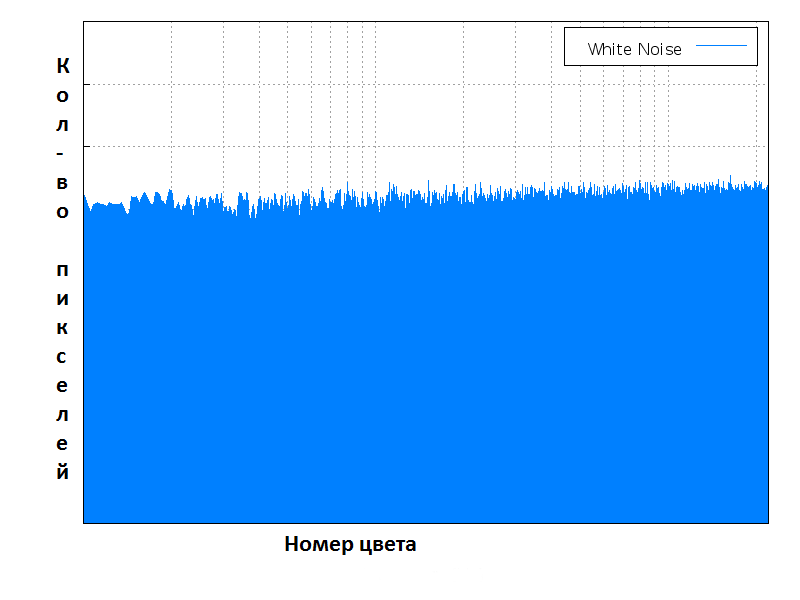
\includegraphics[width=\textwidth]{img/8_white_noise.png}
	\caption{Диаграмма белого шума//почему-то очень много места сверху}
	\label{fig:spire05}
\end{figure}

\subsection{Коричневый шум}
Спектральная плотность коричневого шума пропорциональна 1/f², где f — частота.																									
Это означает, что на низких частотах шум имеет больше энергии, чем на высоких. То есть пикселей темных цветов большей, чем пикселей светлого цвета.Применение фильтра коричневого шума в целом затемняет получаемое изображение.
\\\
\begin{figure}[h]
	\centering
	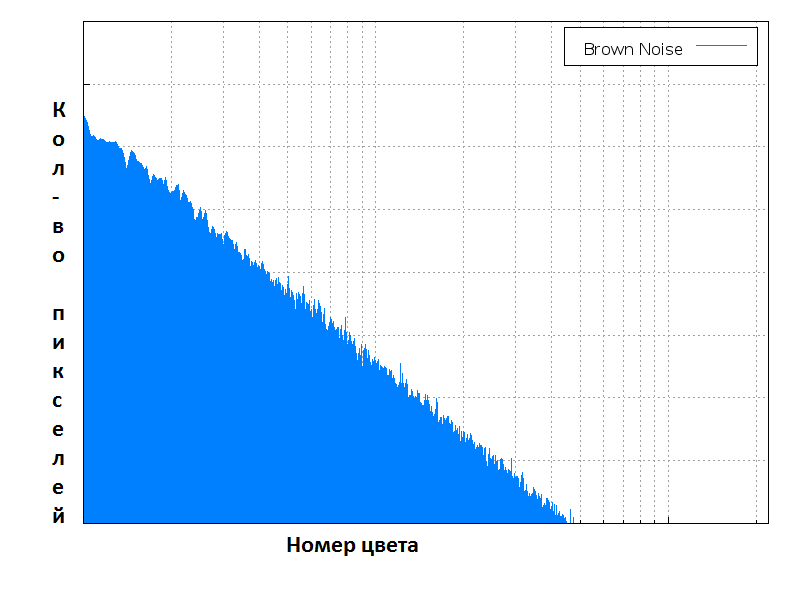
\includegraphics[width=\textwidth ]{img/6_brown_noise.png}
	\caption{Диаграмма красного шума }
	\label{fig:spire04}
\end{figure} 
\begin{lstlisting}[style=pseudocode,caption={Получение коричневого шума}] 
def smoother(noise):
    output = []
    for i in range(len(noise) - 1):
        output.append(0.5 * (noise[i] + noise[i+1]))
return output
\end{lstlisting}

\subsection{Гауссовский шум}

Гауссовский шум  - шум, имеющий функцию плотности вероятности (PDF), равную нормальному распределению, которое также известно как гауссово распределение. 

\begin{equation}
p_g(z)=\frac{1}{\sigma\sqrt{2*\pi}}e^{-\frac{(z-\mu)^2}{2\sigma^2}}
\end{equation}
z - количество цветов, $\mu$ -среднее значение, $\sigma$ - стандартное отклонение.
%\begin{figure}
%	\centering
%  \includegraphics[width=\textwidth]{inc/svg/pic01}
%	\caption{Диаграмма гауссовского шума}
%	\label{fig:spire02}
% \end{figure}
\subsection{Фиолетовый шум}
Фиолетовый  шум представляет собой противооложноть между коричневому шуму. Получение его аналогично получению коричневого шума.Применение фильтра фиолетового шума в целом засветляет получаемое изображение.
\\\\\\\\
\begin{figure}[h!]
	\centering
	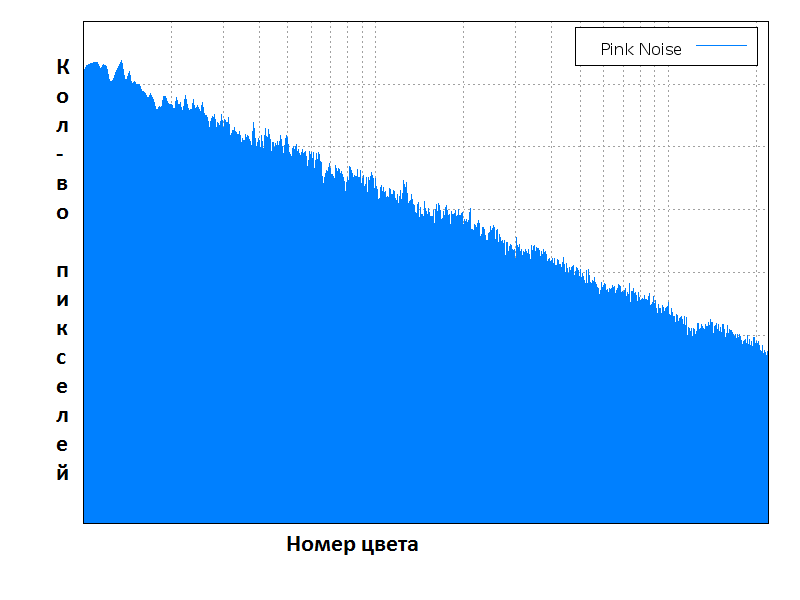
\includegraphics[width=\textwidth]{img/7_pink_noise.png}
	\caption{Диаграмма розового шума}
	\label{fig:spire02}
\end{figure}
\begin{lstlisting}[style=pseudocode,caption={Получение розового шума}]
def rougher(noise):
    output = []
    for i in range(len(noise) - 1):
    output.append(0.5 * (noise[i] - noise[i+1]))
return output
\end{lstlisting}

\subsection{Розовый и синий шумы}
Розовый и синий шумы представляют собой "промежуточные" шумы.Изобржаение с розовым шумом темнее  изображения с белым шумом, но светлее изображения с коричневым шумом. Изображение с синим шумом светлее изображения с белым шумом, но темнее чем изображение с фиолетовым шумом. Их получение аналогично получению со коричневого и фиолетового шумов.

\section{Алгоритм Флойда-Стейнберга}
Рассмотрим более детально алгоритм Флойда-Стейнберга.
P(x,y) - цвет пикселя в точке x,y
I(x,y) - предполгаемый цвет пикселя с учетом ошибки(действительное число)
\begin{figure}[h!]
	\centering
	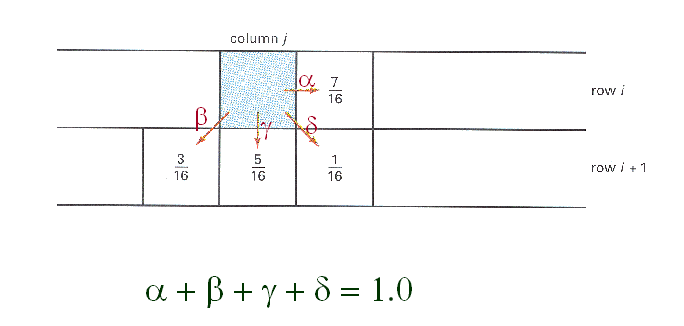
\includegraphics[width=\textwidth]{img/1.png}
	\caption{Схема рассеивания ошибки}
	\label{fig:spire03}
\end{figure}
\begin{lstlisting}[style=pseudocode,caption={Алгоритм Флойда-Стейнберга}]
for x in range(width):
    for y in range(height):
       P(x,y) = trunc(I(x,y)+0.5)
       e = I(x,y) - P(x,y)
       I(x,y+1) += alpha*e
       I(x+1, y-1) += beta*e
       I(x+1, y) += gamma*e
       I(x+1, y+1) += sigma*e
\end{lstlisting}
\section{Комбинация алгоритмов Флойда-Стейнберга и алгоритма случайного распределения}
Комбинируя алгоритмы Флойда-Стейнберга и алгоритм случайнгого распределения, мы, возможно, получим алгоритм, превосходящий их по метрикам SSIM и PSNR.
Идея совмещения заключается в том, что коэффициенты диффузии ошибки вычисляются при помощи генерации элемента последовательти шума. Например, для коэффициента 3/16 и алгоритма белоого шума, можно будет равновероятности получить вместо этого коэффициентв 0/16,1/16,2/16,3/16.\\
Алгоритм комбинации для белого шума, комбинации остальных шумов и алгоритма Флойда-Стейнберга тривиальны и аналогичны. 
\begin{lstlisting}[style=pseudocode,caption={Алгоритм Флойда-Стейнберга и белый шум}]
for x in range(width):
    for y in range(height):
        P(x,y) = trunc(I(x,y)+0.5)
        e = I(x,y) - P(x,y)
        I(x,y+1) += random.randint(1,alpha*16)/16*e
        I(x+1, y-1) += random.randint(1,beta*16)/16*e
        I(x+1, y) += random.randint(1,gamma*16)/16*e
        I(x+1, y+1) +=  random.randint(1,sigma*16)/16*e
\end{lstlisting}


%%% Local Variables:

%%% mode: latex
%%% TeX-master: "rpz"
%%% End:
%--количество цветов
%||количество пикселей